\documentclass[12pt,a4paper]{article}
\usepackage[utf8]{inputenc}
\usepackage[english,russian]{babel}
\usepackage{amssymb,amsfonts,amsmath,cite,enumerate,float,indentfirst}
\usepackage{graphicx}
\usepackage{geometry}
\usepackage{systeme}
\usepackage{hyperref}
\usepackage{url}
\hypersetup{
	colorlinks,
	citecolor=black,
	filecolor=black,
	linkcolor=black,
	urlcolor=black
}
\geometry{left=2cm}
\geometry{right=1.5cm}
\geometry{top=2cm}
\geometry{bottom=2cm}

\begin{document}
	
\begin{titlepage}
	\begin{center}		
		\vfill	
		Санкт-Петербургский политехнический университет \\
		Петра Великого\\
		\vskip 1cm
		Институт прикладной математики и механики \\
		Кафедра «Прикладная математика»
		\vfill
		\textbf{Отчёт\\
			по лабораторным работам №1-4\\
			по дисциплине\\
			«Математическая статистика»\\}
		\vfill
	\end{center}
	\vfill
	\hfill
	\begin{minipage}{0.4\textwidth}
		Выполнил студент:\\
		Самутичев Евгений Романович\\
		группа: 3630102/70201\\
	\end{minipage}
	\vfill
	\hfill 
	\begin{minipage}{0.4\textwidth}
		Проверил:\\
		к.ф.-м.н., доцент\\
		Баженов Александр Николаевич\
	\end{minipage}
	\vfill
	\begin{center}
		Санкт-Петербург\\2020 г.
	\end{center}
\end{titlepage}

\tableofcontents
\listoffigures
\listoftables
\pagebreak

\section{Постановка задачи}
Для каждого из 5 распределений:

\begin{itemize}
	\item Нормального $N(x, 0, 1)$
	\item Коши $C(x, 0, 1)$
	\item Лапласа $L(x, 0, \frac{1}{\sqrt{2}})$
	\item Пуассона $P(k, 10)$
	\item Равномерного $U(x, -\sqrt{3}, \sqrt{3})$	
\end{itemize}

выполнить следующее:
\begin{enumerate}
	\item сгенерировать массив случайных данных (выборку) размера: 10, 50, 1000 и построить графики плотности вероятности (функции вероятности для распределения Пуассона как дискретного).
	
	\item выборку размера: 10, 100, 1000 - сгенерировать 1000 раз, для каждой генерации произвести вычисления выборочных характеристик $\bar x, \text{med }x, z_R, z_Q, z_{tr}$ для всех генераций в рамках одного размера выборки получить значения среднего характеристик положения:
	\begin{equation}\label{1}
		E(z) = \bar z
	\end{equation}
	и дисперсию:
	\begin{equation}\label{2}
		D(z) = \bar {z^2} - {\bar z}^2
	\end{equation}
	Представить полученные данные в виде таблиц.
	
	\item сгенерировать выборки размера 20 и 100, построить боксплот Тьюки. Определить долю выбросов экспериментально (сгенерировав выборку каждого размера 1000 раз) и сравнить с результатами полученными теоретически.
	
	\item сгенерировать выборки размером 20, 60 и 100 элементов. Построить на них эмпирические функции распределения и ядерные оценки плотности/функции распределения на отрезке $[-4, 4]$ для непрерывных распределений и на отрезке $[6,14]$ для распределения Пуассона.
\end{enumerate}

\pagebreak

\section{Теория}
\subsection{Распределения}
Пусть задано вероятностное пространство $(\Omega, \mathcal{F}, \mathbf{P})$, на котором определена \textit{случайная величина} $\xi:\Omega\to\mathbb{R}$ т.е. функция $\xi(\omega)$ такая что $\xi^{-1}(B)\in\mathcal{F},\forall{B\in\mathcal{B}(\mathbb{R})}$. Она индуцирует вероятностную меру на $\mathbb{R}$ как $\mathbf{P}_\xi(B)=\mathbf{P}(\xi^{-1}(B))$ которая и носит название \textit{распределения вероятностей} случайной величины\cite{shiryaev}.

Функция $F_\xi(x)=\mathbf{P}_\xi\mathopen{(-\infty}, x\mathclose{ ] },x\in\mathbb{R}$ называется \textit{функцией распределения} случайной величины $\xi$. Случайная величина может быть:

\begin{enumerate}
	\item \textit{дискретной}, если распределение представимо в виде $\mathbf{P}_\xi(B)=\sum\limits_{k:x_k\in{B}}{p(x_k)}$, где \newline
	$p(x_k)=\mathbf{P}_\xi{\{ x_k \}}$ для конечного $\{x_1, ..., x_n\}$ или счетного 
	$\{x_1, ..., x_k, ...\}$ подмножества вещественных чисел. В этом случае функция $p(x_k)$ называется таблицей распределения.
	
	\item \textit{непрерывной}, если $F(x)$ непрерывна
	
	\item \textit{абсолютно непрерывной}, если существует такая неотрицательная функция $f_\xi(x)$ называемая \textit{плотностью вероятности}, что $F(x)=\int\limits_{-\infty}^{x}{f(y)dy}$
\end{enumerate}

В работе рассматриваются следующие распределения:

\begin{enumerate}
	\item \textit{Нормальное} $N(x, 0, 1)$ - абсолютно непрерывное, задается плотностью
	\begin{equation}
	f_N(x)=\frac{1}{\sqrt{2\pi}}e^{-\frac{x^2}{2}}
	\end{equation}
	
	\item \textit{Коши} $C(x, 0, 1)$ - абсолютно непрерывное, задается плотностью
	\begin{equation}
	f_C(x)=\frac{1}{\pi(x^2+1)}
	\end{equation}
	
	\item \textit{Лапласа} $L(x, 0, \frac{1}{\sqrt{2}})$ - абсолютно непрерывное, задается плотностью
	\begin{equation}
	f_L(x)=\frac{1}{2\sqrt{2}}e^{-\frac{1}{\sqrt{2}}|x|}
	\end{equation}
	
	\item \textit{Пуассона} $P(k, 10)$ - дискретное, задается на $\{1, 2, ..., k, ...\}$ как
	\begin{equation}
	p(k)=\frac{10^k}{k!}e^{-10}
	\end{equation} 
	
	\item \textit{Равномерное} $U(x, -\sqrt{3}, \sqrt{3})$ - абсолютно непрерывное, задается плотностью 
	\begin{equation}
	f_U(x) = 
	\begin{cases}
	\frac{1}{2\sqrt{3}} &\text{если $x \in \mathopen[-\sqrt{3}, \sqrt{3}\mathclose] $}\\
	0 &\text{иначе}
	\end{cases}
	\end{equation}	
\end{enumerate}

\subsection{Гистограмма}
Все приведенные распределения характеризуются таблицей (для дискретных) или плотностью (для абсолютно непрерывных). Эмпирическим аналогом таблицы или плотности является \textit{гистограмма}\cite{chernova}. Гистрограмма строится по группированным данным. Предполагаемую область значений случайной величины $\xi$ делят на некоторое количество интервалов:

Пусть $A_1, ..., A_k$ - интервалы на прямой. Обозначим $\nu_j,j\in\{1, ..., k\}$ - число элементов выборки, попавших в интервал $A_j$. Размер выборки в этих обозначениях равен $n=\sum\limits_{j=1}^{k}{\nu_j}$. На каждом из интервалов строят прямоугольник, площадь которого пропорциональна $\nu_j$, общая площадь всех прямоугольников должна равняться единице (нормировка гистограммы), поэтому высота каждого определяется как $f_j=\frac{\nu_j}{nl_j}$. Полученная фигура из объединения прямоугольников и называется гистограммой.

\subsection{Вариационный ряд}
Если элементы выборки $x_1, ..., x_n$ упорядочить по возрастанию на каждом элементарном исходе (рассматриваем их как случайные величины), получится новый набор случайных величин, называемый \textit{вариационным рядом}:
$$x_{(1)} \leq ... \leq x_{(n)}$$ Элемент $x_{(k)}$ называется \textit{k-ой порядковой статистикой}
\footnote{\cite{chernova} стр. 10} .

\subsection{Выборочные характеристики}
При работе с выборкой нам неизвестно распределение по которому она получена, а значит и соответствующие характеристики распределения. Однако, существуют оценки - т.н. \textit{выборочные характеристики}:

\begin{itemize}
	\item Выборочное среднее
	\begin{equation}\label{8}
	\bar x = \frac{1}{n}\sum_{i=1}^{n}{x_i}
	\end{equation}
	
	\item Выборочная медиана
	\begin{equation}\label{9}
	\text{med }x = 
	\begin{cases}
	x_{(k+1)} &\text{при $n=2k+1$}\\
	\frac{x_{(k)} + x_{(k+1)}}{2} &\text{при $n=2k$}
	\end{cases}
	\end{equation}
	
	\item Полусумма экстремальных выборочных элементов
	\begin{equation}\label{10}
	z_R = \frac{x_{(1)} + x_{(n)}}{2}
	\end{equation}
	
	\item Выборочный квантиль уровня $\alpha$
	\begin{equation}
	z_{\alpha} = \frac{x_{(\lfloor q \rfloor+1)} +
		x_{(\lceil q \rceil+1)}}{2}, \text{где } q=(n-1)\alpha
	\end{equation}
	формула, используемая в \textbf{NumPy}, в этом случае $z_0 = \min\limits_{i=1,...,n}x_{(i)}, z_1 = \max\limits_{i=1,...,n}x_{(i)},
	\newline z_{0.5} = \text{med} \hspace{2pt} x$
	
	\item Полусумма квантилей
	\begin{equation}\label{12}
	z_Q = \frac{z_{0.25} + z_{0.75}}{2}
	\end{equation}
	
	\item Усеченное среднее
	\begin{equation}\label{13}
	z_{tr} = \frac{1}{n-2r}\sum_{i=r+1}^{n-r}x_{(i)}, \text{где } r=\lceil \frac{n}{4} \rceil
	\end{equation}
\end{itemize}

Выборочные характеристики как борелевские функции от случайных величин (выборки) также являются случайными величинами, поэтому в работе и производится усреднение их значений для 1000 генераций и вычисление дисперсии.

\subsection{Выбросы}
\subsubsection{Определение}
Результат измерения, выделяющийся из выборки называется \textit{выбросом}. Простейший критерий основан на межквартильном расстоянии, выбросами считаются элементы выборки лежащие вне диапазона $[X_1, X_2]$:
\begin{equation}\label{14}
X_1=LQ - \frac{3}{2}(UQ-LQ), X_2=UQ + \frac{3}{2}(UQ-LQ)
\end{equation}, где $LQ, UQ$ - выборочные нижний и верхний квартили.

Теоретическая вероятность выбросов для непрерывных распределений:
\begin{equation}\label{15}
P_{outlier} = P(x<X_1) + P(x>X_2) = F(X_1) + (1 - F(X_2))
\end{equation}
, а для дискретных с учетом возможного скачка
\begin{equation}\label{16}
P_{outlier} = F(X_1) - (F(X_1+) - F(X_1)) + (1 - F(X_2))
\end{equation}

\subsubsection{Доля выбросов}
Проведем следующий эксперимент $1,...,i,...,N$ раз: сгенерируем выборку размера $n$ и подсчитаем число выбросов $k_i$, используя определение \hyperref[1]{(1)}, но с выборочными квартилями. Тогда доля выбросов в $i$-м эксперименте:
\begin{equation}
P_i = \frac{k_i}{n}
\end{equation}

Собственно \textit{долей выбросов} будем называть величину
\begin{equation}\label{17}
P = \frac{1}{N}\sum_{i=1}^{N} P_i
\end{equation},
с дисперсией
\begin{equation}\label{18}
D = \frac{1}{N}\sum_{i=1}^{N} P_i^2 - P^2
\end{equation}

\subsection{Боксплот Тьюки}
\subsubsection{Описание}
\textit{Боксплот} (англ. box plot) — график, использующийся в описательной статистике, компактно изображающий одномерное распределение вероятностей: в удобной форме показывает медиану, нижний и верхний квартили, минимальное и максимальное значение выборки и выбросы.\cite{boxplot}

\subsubsection{Построение}
Границами ящика служат $LQ \text{ и } UQ$, линия в середине ящика — медиана. Концы усов — края статистически значимой выборки (без выбросов): $X_1 \text{ и } X_2 \text{ }\hyperref[1]{(1)}$.

\subsection{Эмпирическая функция распределения}
\textit{Эмпирической функцией распределения}, построенной по выборке $(x_1, ..., x_n)$ объема $n$ называется случайная функция $F_n^*: \mathbb{R} \times \Omega \to [0,1]$, которая имеет вид

\begin{equation}
F_n^*(y) = \frac{1}{n}\sum_{i=1}^n{I(x_i < y)}
\end{equation}
где $I$ - индикатор события $x_i < y$\cite{chernova}

\subsection{Ядерная оценка плотности распределения}
Пусть $(x_1, ..., x_n)$ - выборка полученная по распределению с некоторой плотностью $f$, требуется оценить функцию $f$. \textit{Ядерным оценщиком плотности} называется\cite{kde}

\begin{equation}
\hat{f}_h(x) = \frac{1}{nh}\sum_{i=1}^{n}{K\left(\frac{x-x_i}{h}\right)}
\end{equation}
где $K$ - т.н. \textit{ядро} (некоторая неотрицательная функция), $h>0$ - сглаживающий параметр, именуемый \textit{шириной полосы}.
\newline

Как правило используется нормальное (или гауссово) ядро, в силу его удобных математических свойств:
\begin{equation}
K(x) = \frac{1}{\sqrt{2\pi}}e^{-\frac{x^2}{2}}
\end{equation}
\newline
\label{silverman}
В случае если используется гауссово ядро и оцениваемая плотность является гауссовой, оптимальный выбор для $h$ определяется т.н. \textit{правилом Сильвермана}\cite{kde}:
\begin{equation}
h_n = \left(\frac{4s_n^5}{3n}\right)^{\frac{1}{5}}\approx 1.06s_n n^{-\frac{1}{5}}
\end{equation}
где $s_n$ - выборочное среднеквадратичное отклонение (корень из выборочной дисперсии)

\pagebreak

\section{Реализация}
Работа выполнена с использованием языка \textbf{Python} в интегрированной среде разработки \textbf{PyCharm}, были задействованы библиотеки:

\begin{itemize}
	\item \textbf{NumPy} - работа с массивами данных, построение вариационного ряда и вычисления характеристик, вычисление квартилей для дальнейшего подсчета выбросов
	\item \textbf{SciPy} - модуль \textbf{stats} для генерации данных по распределениям, вычисления ядерной оценки плотности
	\item \textbf{Matplotlib} - отрисовка гистограмм и графиков, построение боксплотов
\end{itemize}
\pagebreak

\section{Результаты}
\subsection{Гистограммы и графики}
\begin{figure}[h!]
	\centering
	\includegraphics[scale=0.8]{histogram/normal.png}
	\caption{Нормальное распределение}
	\label{fig:image}
\end{figure}

\begin{figure}[h!]
	\centering
	\includegraphics[scale=0.8]{histogram/cauchy.png}
	\caption{Распределение Коши}
	\label{fig:image}
\end{figure}

\pagebreak

\begin{figure}[h!]
	\centering
	\includegraphics[scale=0.8]{histogram/laplace.png}
	\caption{Распределение Лапласа}
	\label{fig:image}
\end{figure}

\begin{figure}[h!]
	\centering
	\includegraphics[scale=0.8]{histogram/poisson.png}
	\caption{Распределение Пуассона}
	\label{fig:image}
\end{figure}

\pagebreak

\begin{figure}[h!]
	\centering
	\includegraphics[scale=0.8]{histogram/uniform.png}
	\caption{Равномерное распределение}
	\label{fig:image}
\end{figure}
\pagebreak

\subsection{Выборочные характеристики}
\begin{table}[h!]
	\centering
	\begin{tabular}{|l|l|l|l|l|l|}
		\hline&$\bar x\text{	} \hyperref[8]{(8)}$ &$\text{med }x\text{	} \hyperref[9]{(9)}$  &$z_R\text{	} \hyperref[10]{(10)}$  &$z_Q\text{	} \hyperref[12]{(12)}$  &$z_{tr}\text{	} \hyperref[13]{(13)}$  \\ \hline
		$n=10$&&&&& \\ \hline$E(z)$&-0.0&-0.0&-0.0&-0.0&-0.1 \\ \hline$D(z)$&0.094467&0.130519&0.187448&0.105385&0.069492 \\ \hline
		
		$n=100$&&&&& \\ \hline$E(z)$&0.0&0.0&0.0&0.01&-0.01 \\ \hline$D(z)$&0.009651&0.015116&0.091466&0.011977&0.011309 \\ \hline
		
		$n=1000$&&&&& \\ \hline$E(z)$&-0.0&0.001&0.0&-0.0&-0.001 \\ \hline$D(z)$&0.001049&0.00153&0.062347&0.001313&0.001193 \\ \hline
		
	\end{tabular}
	\caption{Нормальное распределение}
\end{table}

\begin{table}[h!]
	\centering
	\begin{tabular}{|l|l|l|l|l|l|}
		\hline&$\bar x$ &$\text{med }x$  &$z_R$  &$z_Q$  &$z_{tr}$  \\ \hline
		$n=10$&&&&& \\ \hline$E(z)$&-0.0&-0.0&-1.0&-0.0&-0.2 \\ \hline$D(z)$&490.607293&0.332166&11914.643438&1.132547&0.210165 \\ \hline
		
		$n=100$&&&&& \\ \hline$E(z)$&2.0&0.0&79.0&0.0&-0.01 \\ \hline$D(z)$&3581.697241&0.026278&8922533.221739&0.04842&0.025421 \\ \hline
		
		$n=1000$&&&&& \\ \hline$E(z)$&1.0&0.0&642.0&0.0&-0.0 \\ \hline$D(z)$&2223.205146&0.00256&547218440.611133&0.004966&0.002619 \\ \hline
	\end{tabular}
	\label{tab:cauchy}
	\caption{Распределение Коши}
\end{table}

\begin{table}[h!]
	\centering
	\begin{tabular}{|l|l|l|l|l|l|}
		\hline&$\bar x$ &$\text{med }x$  &$z_R$  &$z_Q$  &$z_{tr}$  \\ \hline
		$n=10$&&&&& \\ \hline$E(z)$&0.0&0.0&0.0&0.0&-0.1 \\ \hline$D(z)$&0.098335&0.072722&0.382323&0.089897&0.041919 \\ \hline
		
		$n=100$&&&&& \\ \hline$E(z)$&-0.0&0.0&-0.0&-0.0&-0.01 \\ \hline$D(z)$&0.009719&0.00561&0.433362&0.009396&0.005806 \\ \hline
		
		$n=1000$&&&&& \\ \hline$E(z)$&0.0&0.001&-0.0&0.001&-0.0 \\ \hline$D(z)$&0.000918&0.000483&0.441511&0.000944&0.000561 \\ \hline
	\end{tabular}
	\caption{Распределение Лапласа}
\end{table}

\pagebreak

\begin{table}[h!]
	\centering
	\begin{tabular}{|l|l|l|l|l|l|}
		\hline&$\bar x$ &$\text{med }x$  &$z_R$  &$z_Q$  &$z_{tr}$  \\ \hline
		$n=10$&&&&& \\ \hline$E(z)$&10.0&10.0&10.0&10.0&7.0 \\ \hline$D(z)$&0.955624&1.3806&1.744716&1.128935&0.704541 \\ \hline
		
		$n=100$&&&&& \\ \hline$E(z)$&10.0&9.9&11.0&9.9&9.6 \\ \hline$D(z)$&0.097956&0.194391&0.997104&0.14328&0.110723 \\ \hline
		
		$n=1000$&&&&& \\ \hline$E(z)$&10.0&10.0&12.0&9.994&9.84 \\ \hline$D(z)$&0.010385&0.003484&0.6581&0.002748&0.011585 \\ \hline
	\end{tabular}
	\caption{Распределение Пуассона}
\end{table}

\begin{table}[h!]
	\centering
	\begin{tabular}{|l|l|l|l|l|l|}
		\hline&$\bar x$ &$\text{med }x$  &$z_R$  &$z_Q$  &$z_{tr}$  \\ \hline
		$n=10$&&&&& \\ \hline$E(z)$&0.0&0.0&-0.0&0.0&-0.1 \\ \hline$D(z)$&0.10033&0.234165&0.043909&0.136123&0.119729 \\ \hline
		
		$n=100$&&&&& \\ \hline$E(z)$&0.0&-0.0&0.001&0.0&-0.02 \\ \hline$D(z)$&0.009457&0.028559&0.00059&0.014028&0.018067 \\ \hline
		
		$n=1000$&&&&& \\ \hline$E(z)$&-0.001&-0.002&4e-05&-0.001&-0.003 \\ \hline$D(z)$&0.00102&0.003073&6e-06&0.001465&0.002005 \\ \hline
	\end{tabular}
	\caption{Равномерное распределение}
\end{table}
\pagebreak

\subsection{Боксплоты}
\begin{figure}[h!]
	\centering
	\includegraphics[scale=0.8]{boxplot/normal.png}
	\caption{Нормальное распределение}
	\label{fig:image}
\end{figure}

\begin{figure}[h!]\label{4}
	\centering
	\includegraphics[scale=0.8]{boxplot/cauchy.png}
	\caption{Распределение Коши}
	\label{fig:image:cauchy}
\end{figure}

\pagebreak

\begin{figure}[h!]
	\centering
	\includegraphics[scale=0.8]{boxplot/laplace.png}
	\caption{Распределение Лапласа}
	\label{fig:image}
\end{figure}

\begin{figure}[h!]
	\centering
	\includegraphics[scale=0.8]{boxplot/poisson.png}
	\caption{Распределение Пуассона}
	\label{fig:image}
\end{figure}

\pagebreak

\begin{figure}[h!]
	\centering
	\includegraphics[scale=0.8]{boxplot/uniform.png}
	\caption{Равномерное распределение}
	\label{fig:image}
\end{figure}
\pagebreak

\subsection{Теоретическая вероятность выбросов}
Подсчитана для каждого распределения при помощи модуля {stats} библиотеки {SciPy} (см. \hyperref[sec:impl]{Реализация}):

\begin{table}[h!]
	\centering
	\begin{tabular}{|l|l|l|l|l|l|}
		\hline
		Распределение&normal&cauchy&laplace&poisson&uniform  \\ \hline
		$P_{outlier}\text{	} \hyperref[15]{(15)},\hyperref[16]{(16)}$
		&0.007  &0.156  &0.0625  &0.008  &0.0  \\ \hline
	\end{tabular}
	\caption{Теоретическая вероятность выбросов}
\end{table}

\subsection{Доля выбросов}
\begin{table}[h!]
	\centering
	\begin{tabular}{|l|l|l|l|l|l|}
		\hline
		Распределение&normal&cauchy&laplace&poisson&uniform  \\ \hline
		$n=20$& & & & & \\ \hline
		$P\hyperref[18]{(18)}$&0.025 &0.147 &0.070 &0.022 &0.0023  \\ \hline
		$D\hyperref[19]{(19)}$&0.002085 &0.005248 &0.004219 &0.001801 &0.0002  \\ \hline
		$n=100$& & & & & \\ \hline
		$P$&0.0105 &0.156 &0.0658 &0.0108 &0.0  \\ \hline
		$D$&0.000185 &0.001068 &0.0009 &0.000236 &0.0 \\ \hline
	\end{tabular}
	\caption{Доля выбросов}
\end{table}

\subsection{Эмпирические функции распределения}
\begin{figure}[h!]
	\centering
	\includegraphics[scale=0.8]{ecdf/normal.png}
	\caption{Нормальное распределение}
	\label{fig:image}
\end{figure}

\begin{figure}[h!]
	\centering
	\includegraphics[scale=0.8]{ecdf/cauchy.png}
	\caption{Распределение Коши}
	\label{fig:image}
\end{figure}
\pagebreak

\begin{figure}[h!]
	\centering
	\includegraphics[scale=0.8]{ecdf/laplace.png}
	\caption{Распределение Лапласа}
	\label{fig:image}
\end{figure}

\begin{figure}[h!]
	\centering
	\includegraphics[scale=0.8]{ecdf/poisson.png}
	\caption{Распределение Пуассона}
	\label{fig:image}
\end{figure}
\pagebreak

\begin{figure}[h!]
	\centering
	\includegraphics[scale=0.8]{ecdf/uniform.png}
	\caption{Равномерное распределение}
	\label{fig:image}
\end{figure}
\pagebreak

\subsection{Ядерные оценки плотности распределения}
\begin{figure}[h!]
	\centering
	\includegraphics[scale=0.8]{kde/normal.png}
	\caption{Нормальное распределение}
	\label{fig:image}
\end{figure}
\pagebreak

\begin{figure}[h!]
	\centering
	\includegraphics[scale=0.8]{kde/cauchy.png}
	\caption{Распределение Коши}
	\label{fig:image}
\end{figure}
\pagebreak

\begin{figure}[h!]
	\centering
	\includegraphics[scale=0.8]{kde/laplace.png}
	\caption{Распределение Лапласа}
	\label{fig:image}
\end{figure}
\pagebreak

\begin{figure}[h!]
	\centering
	\includegraphics[scale=0.8]{kde/poisson.png}
	\caption{Распределение Пуассона}
	\label{fig:image}
\end{figure}
\pagebreak

\begin{figure}[h!]
	\centering
	\includegraphics[scale=0.8]{kde/uniform.png}
	\caption{Равномерное распределение}
	\label{fig:image}
\end{figure}
\pagebreak

\section{Обсуждение}
\subsection{Гистограммы и графики}
Проведенный эксперимент подтверждает \textbf{утверждение}: \textit{пусть плотность распределения по которому построена выборка является непрерывной функцией. Если число интервалов гистограммы $k(n)$ стремится к бесконечности таким образом что $\lim\limits_{n\to\infty}{\frac{k(n)}{n}}=0$, то имеет место сходимость по вероятности гистограммы к плотности.}\cite{chernova} Действительно мы взяли $k(n)=\lceil\sqrt{n}\rceil$ и очевидно условие утверждения в таком случае выполнено, при этом гистограмма при увеличении $n$ заполняет площадь под графиком плотности (кусочно-линейной функции вероятности для распределения Пуассона), а это и означает сходимость по вероятности.

\subsection{Математическое ожидание и медиана}
Для каждого из указанных в постановке задачи распределений, приведем теоретические значения математического ожидания и медианы:

\begin{itemize}
	\item $N(x, 0, 1): \mathbf{E}=0, \text{med}=0$ 
	\item $C(x, 0, 1): \mathbf{E} - \text{не определено}, \text{med}=0$
	\item $L(x, 0, \frac{1}{\sqrt{2}}): \mathbf{E}=0, \text{med}=0$
	\item $P(k, 10): \mathbf{E}=10, \text{med}=10$
	\item $U(x, -\sqrt{3}, \sqrt{3}): \mathbf{E}=0, \text{med}=0$
\end{itemize}

Как известно, \textit{выборочное среднее является несмещенной и состоятельной оценкой для математического ожидания}\footnote{\cite{chernova} стр. 17} Это объясняет то что для всех распределений кроме распределения Коши - выборочное среднее при росте $n$ стремится к математическому ожиданию, для распределения Коши последовательность вычислений не демонстрирует никакой сходимости (см. \hyperref[tab:cauchy]{таблицу 2}), поскольку у него отсутствует математическое ожидание. В тоже время медиана имеется у всех распределений и к ней сходится выборочная медиана.

\subsection{Полусуммы: $z_R$ и $z_Q$}
Полусумма квартилей $z_Q$ и экстремальных выборочных элементов $z_R$ оценивают центр симметрии распределения, из таблиц наблюдается что $z_Q$ ближе к медиане и последовательность вычислений $E(z) \text{ для } z_Q$ при увеличении $n$ сходится, в тоже время последовательность значений $E(z) \text{ для } z_R$ расходится при распределении Коши. Таким образом оценка через полусумму квартилей лучше, хотя и требует больше вычислений.

\subsection{Упорядочение характеристик}
Для $n=1000$ приведем упорядочение характеристик положения по каждому распределению:
\begin{itemize}
	\item $N(x, 0, 1): z_{tr} < z_Q \leq \bar x \leq z_R < \text{med }x$
	\item $C(x, 0, 1): z_{tr} \leq z_Q \leq \text{med }x < \bar x < z_R$
	\item $L(x, 0, \frac{1}{\sqrt{2}}): z_{tr} \leq z_R \leq \bar x < \text{med }x \leq z_Q$
	\item $P(k, 10): z_{tr} < z_Q < \text{med }x \leq \bar x < z_R$
	\item $U(x, -\sqrt{3}, \sqrt{3}): z_{tr} < \text{med }x < z_Q \leq \bar x < z_R$
\end{itemize}

\subsection{Выбросы}
Из полученных таблиц видно что доля выбросов близка к теоретической. Наибольшая при этом у распределения Коши, что также видно по боксплоту Тьюки \hyperref[fig:image:cauchy]{(рис. 7)}. Вторая по величине у распределения Лапласа. Для остальных выборок доля выбросов не превосходит $95\%$, а значит можно считать что они соответствуют гипотетическим распределениям.

\subsection{Эмпирическая функция распределения}
Существует \textbf{теорема} \cite{chernova}: \textit{Пусть $(x_1, ..., x_n)$ - выборка из распределения с некоторой функцией распределения $F$ и пусть $F_n^*$ - эмпирическая функция распределения построенная по этой выборке. Тогда $F_n^*(y) \overset{p}{\to} F(y), \forall y \in \mathbb{R}$} Полученные графики подтверждают данный теоретический факт, с ростом $n$ эмпирическая функцяи распределения все ближе к истинной. 

\subsection{Ядерная оценка плотности распределения}
Для нормального распределения наилучшие результаты показал выбор $h$ по правилу Сильвермана, что обосновано теоретически т.к. он оптимален в некотором смысле (см. \hyperref[silverman]{Теория}), как и для распределения Пуассона. Для распределения Лапласа хорошие результаты в приближении плотности распределения имеем как при $h_n$, так и при $0.5h_n$. Плотность равномерного распределения аппроксимируется неудачно т.к. оно далеко от гауссова, как и распределение Коши.

\pagebreak

\section{Приложения}
\noindent 1. Исходный код лабораторной 1 {\url{https://github.com/zhenyatos/statlabs/tree/master/Lab1}} \\
\noindent 2. Исходный код лабораторной 2  {\url{https://github.com/zhenyatos/statlabs/tree/master/Lab2}} \\
\noindent 3. Исходный код лабораторной 3  {\url{https://github.com/zhenyatos/statlabs/tree/master/Lab3}} \\
\noindent 4. Исходный код лабораторной 4 {\url{https://github.com/zhenyatos/statlabs/tree/master/Lab4}}

\begin{thebibliography}{9} 
	\addcontentsline{toc}{section}{Список литературы}
	\bibitem{shiryaev} А. Н. Ширяев, \emph{Вероятность-1}. Изд. МЦНМО, Москва, 2017. 551 стр. 
	
	\bibitem{chernova} Н. И. Чернова, \emph{Математическая статистика: Учеб. пособие}. Новосиб. гос. ун-т. Новосибирск, 2007. 148 стр.
	
	\bibitem{boxplot} Ящик с усами // Википедия. [2020—2020]. Дата обновления: 12.01.2020. URL: \url{https://ru.wikipedia.org/?oldid=104502300} (дата обращения: 12.01.2020)
	
	\bibitem{kde} Ядерная оценка плотности // Википедия. [2020—2020]. Дата обновления: 05.01.2020. URL: https://ru.wikipedia.org/?oldid=104368872 (дата обращения: 05.01.2020).
\end{thebibliography}

\end{document}
